%
%%%%%%%%%%%%%%%%%%%%%%%%%%%%%%%%%%%%%%%%%%%%%%%%%%%%%%%%%%%%%%%%%%%%%%%%%%%%%%%%
\chapter{Theoretical background}\label{chap:1}
%%%%%%%%%%%%%%%%%%%%%%%%%%%%%%%%%%%%%%%%%%%%%%%%%%%%%%%%%%%%%%%%%%%%%%%%%%%%%%%%
%

%
%%%%%%%%%%%%%%%%%%%%%%%%%%%%%%%%%%%%%%%%%%%%%%%%%%%%%%%%%%%%%%%%%%%%%%%%%%%%%%%%
\section{Introduction}\label{sec:intro}
%%%%%%%%%%%%%%%%%%%%%%%%%%%%%%%%%%%%%%%%%%%%%%%%%%%%%%%%%%%%%%%%%%%%%%%%%%%%%%%%
%
Many crystals with a lack of inversion symmetry show an interesting phase
consisting of a regular arrangement of magnetic whirl tubes called skyrmions.
These spin configurations are found in a wide range of chiral
magnets~\cite{skyrm1, skyrm2, skyrm3, skyrm4, skyrm5, skyrm6, Milde, skyrm8,
skyrm9, skyrm10} and have received a lot of attention lately mostly due to the
topological stability of a quantized winding number associated with the whirl
tubes. Defect mobility or skyrmion switching~\cite{switch} might make them
suitable candidates for a permanent fast and efficient memory or other
spintronic devices.

Besides direct observation through a variety of experimental techniques, numeric
simulations have contributed significantly to the understanding of
skyrmions~\cite{skyrmion, Milde, switch}. The typical setup is a
three-dimensional spin lattice with a discretized Hamiltonian consisting of
direct exchange, an external field Zeeman term and the weak
Dzyaloshinskii-Moriya interaction. In Monte Carlo simulations one can observe
the helical, conical and skyrmion phase and, even more interestingly, observe
time resolved phase transitions. The goal of this report was to implement such a
Monte Carlo code and reproduce results by Buhrandt and Fritz~\cite{skyrmion},
\ie{} observe the three different phases and search for phase transitions by
repeated sampling at different temperatures and external fields. Furthermore we
observe the disappearance of skyrmions both into the fully ordered phase and
into the helical phase by dynamically increasing or decreasing the magnetic
field respectively as described and observed in~\cite{Milde} \todo{back paper
ausknipsen}.

Since most of the limited time designated for this project was spent on the
implementation and verification of the Monte Carlo code with simulated annealing
and the Metropolis algorithm, we split this work into two parts. The first one
provides a general introduction to Monte Carlo methods and describes all
algorithmic aspects in great detail. While the lattice model is referred to as
a specific example, we do not discuss the physical consequences in detail there.
The present complementary report on the other hand describes the results of the
simulations without much explanation of the computational methods. Apparently, a
theoretic introduction to the lattice model and interactions cannot be absent in
any of the two. Therefore, \secref{sec:lattice} and \secref{sec:interactions} as
well as \secref{sec:hamiltonian} inevitably have quite some overlap with the
introductory sections of the previous report \emph{Sky-MoCa -- Introduction to
Monte Carlo Methods by Example}.

After that basic introduction, we describe the physical observables and possible
diagnostic techniques to analyze the output of the simulations in
\secref{sec:analysis}. This concludes our theoretical introduction and we
continue in \chapref{chap:2} by first sampling the phase space for different
temperatures and external fields in \secref{sec:phases}, where we will encounter
the helical, conical and skyrmion phase. In \secref{sec:details} we explore the
thermodynamic signature of the helimagnetic phase transition by means of the
specific heat and susceptibility. Eventually, we discuss the transitions from
the skyrmion phase to the helical as well as the totally ordered phase in
\secref{sec:transitions} before we conclude in \secref{sec:conclusion}.
%
%%%%%%%%%%%%%%%%%%%%%%%%%%%%%%%%%%%%%%%%%%%%%%%%%%%%%%%%%%%%%%%%%%%%%%%%%%%%%%%%
\section{The Spin Lattice Model}\label{sec:lattice}
%%%%%%%%%%%%%%%%%%%%%%%%%%%%%%%%%%%%%%%%%%%%%%%%%%%%%%%%%%%%%%%%%%%%%%%%%%%%%%%%
%
A common high-level way to think about magnetism in condensed matter is in terms
of complex collective behavior of spins, each of which is associated with a
magnetic moment. Astoundingly, this figuratively simple model is quite powerful
and allows for a thorough explanation of a wide range of phenomena. Let us
consider a three-dimensional lattice with equidistant spacing in each direction.
To each lattice site we attach a spin, represented by an element of the unit
sphere~$S^2$, see \figref{fig:s2}. In the following we will often resort to the
two-dimensional model for illustration purposes, because it is easier to draw on
a two-dimensional surface as illustrated in \figref{fig:lattice}. However, all
computations solely concern the three-dimensional model. Each vertex of the
lattice could for example represent a nucleus in a solid with a rigid crystal
like structure. Hence the whole lattice can be interpreted as the regular atomic
structure of a simple cubical piece of solid material.

However, we will eventually model chiral magnets like MnSi or
Fe$_\text{1-x}$Co$_\text{x}$Si which in reality are not well modeled by a
homogeneous simple cubic lattice. Therefore, the correspondence between lattice
sites and distinguished physical atoms or electrons must not be taken too
literally. We will elaborate on this point in \secref{sec:hamiltonian}, when we
introduce the continuum model.

\begin{figure}
  \centering
  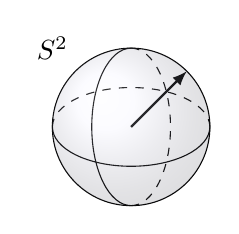
\begin{tikzpicture}
    \draw[->, thick, \select, >=latex] (0,0) -- (45:1cm);
    \draw (-1,0) arc (180:360:1cm and 0.5cm);
    \draw[dashed] (-1,0) arc (180:0:1cm and 0.5cm);
    \draw (0,1) arc (90:270:0.5cm and 1cm);
    \draw[dashed] (0,1) arc (90:-90:0.5cm and 1cm);
    \draw (0,0) circle (1cm);
    \shade[ball color=blue!10!white,opacity=0.20] (0,0) circle (1cm);
    \node at (-1,1) {$S^2$};
  \end{tikzpicture}%
  \caption{We consider three-dimensional spins, \ie{} elements of the unit
  sphere~$S^2$.}
\label{fig:s2}
\end{figure}

\begin{figure}
  \centering
  \begin{tikzpicture}
    \latticeinter{4}
    \begin{scope}[xshift=8cm,yshift=1cm]
      \lattice{4}
    \end{scope}
  \end{tikzpicture}%
  \caption{On the left side we show a two-dimensional spin lattice. Each lattice
  site carries a magnetic moment or spin, represented by an arrow of unit
  length, \ie{}, in the two-dimensional picture, by an element of~$S^1$. The
  neighbors of a lattice site are the ones above, below, left and right in the
  two-dimensional case. The blue squares are the neighbors of the red circle.
  The three-dimensional picture on the right side becomes unclear in a
  two-dimensional drawing rather quickly. Note that the magnetic moments are now
  also three-dimensional, \ie{} elements of the two-dimensional unit
  sphere~$S^2$. In three dimensions each vertex has up to six neighbors.}
\label{fig:lattice}
\end{figure}

We work with a cubic lattice
%
\begin{equation}
  \Sigma := \numlist{1}{N_x} \times \numlist{1}{N_y} \times
  \numlist{1}{N_z} \subset \bN^3 \subset \bR^3\:,
\end{equation}
%
where we interpret~$(i,j,k) \in \Sigma$ as~$i \hx + j \hy + k \hz
\in \bR^3$. Here,~$\hx, \hy, \hz$ are the standard basis vectors of~$\bR^3$.
Note that we can translate the whole lattice by arbitrary integer linear
combinations of the standard basis vectors, thus starting at~$(1,1,1)$ does not
have any physical meaning. It merely corresponds nicely to the numerical
implementation in any~$1$-indexed programming language. At each point~$\r \in
\Sigma$ we attach a spin~$\S_{\r} \in S^2$, which yields the overall
configuration space
%
\begin{equation}
  \Pi := \prod_{\r \in \Sigma} S^2\:.
\end{equation}
%
Each element of~$\Pi$ consists of~$\abs{\Sigma}=N_x N_y N_z$ spins and thus
describes one possible configuration of the whole system. We refer to the
specific spin at position~$\r \in \Sigma$ by~$\S_{\r} \in S^2$. Note that only
the positions of the spins are discretized, but not explicitly their directions.
In any real implementation there is always a fine grained discretization caused
by the finite number of representable floating point numbers. Discrete vertices
and continuous spins mirror nicely the natural crystal structure of solids.

We are going to treat this system thermodynamically by means of the Metropolis
algorithm. The macroscopic observables we are particularly interested in are the
energy, the magnetization, the specific heat and the susceptibility. While there
is a certain similarity to the well known Ising model, there is also a distinct
difference. Our model is in the universality class of short ranged interactions,
not only in three spatial dimensions, but also with a three-dimensional order
parameter, namely the magnetization, with its associated symmetries. At the time
of writing, such systems have not been solved analytically, thus it takes great
efforts to explore phase transitions and their critical exponents. This is
especially true for Monte Carlo simulations, since the correlation length
diverges near the critical temperature, which aggravates computing independent
samples and results in critical slowing of the simulation. This practical issue
will recur in the second chapter.
%
%%%%%%%%%%%%%%%%%%%%%%%%%%%%%%%%%%%%%%%%%%%%%%%%%%%%%%%%%%%%%%%%%%%%%%%%%%%%%%%%
\section{Interactions}\label{sec:interactions}
%%%%%%%%%%%%%%%%%%%%%%%%%%%%%%%%%%%%%%%%%%%%%%%%%%%%%%%%%%%%%%%%%%%%%%%%%%%%%%%%
%
\subsubsection{Ferromagnetic/direct exchange}

The most obvious interaction is the \newterm{ferromagnetic} or \newterm{direct}
exchange. Pictorially speaking, it favors constellations where spins that are
close to each other point into the same direction. A system only interacting
this way will end up in a state where all spins are parallel to each other. The
measure for parallelism of two neighboring spins~$\S_{\r_1}, \S_{\r_2} \in S^2$
can be expressed as
%
\begin{equation}
  -\S_{\r_1} \cdot \S_{\r_2} =
  -\norm{\S_{\r_1}} \norm{\S_{\r_2}} \cos(\alpha) \:,
\end{equation}
%
where~$\alpha$ is the angle between~$\S_{\r_1}$ and~$\S_{\r_2}$. The minus sign
ensures that the energy of two parallel spins is actually smaller than the
energy of two perpendicular or even antiparallel ones. While easily
comprehensible theoretically, in real materials it is far from obvious whether
the direct exchange between localized magnetic moments at different lattice
sites is indeed such a prevalent interaction. For many elements like rare earths
the unpaired 4f electrons are close to the nucleus and cannot remotely extend
out to the orbitals of neighboring atoms. Even the 3d orbitals of transition
metals such as the ferromagnetic Fe, Ni and Co, which extend further from the
nucleus the overlap is barely sufficient to base all magnetic properties on
direct exchange. For metals one would have to account for conduction electrons
and the band structure of course.

Again this encourages the viewpoint that the lattice~$\Sigma$ does not represent
the atomic crystal structure, but is merely a discretized version of a
continuous model. In this sense the ferromagnetic exchange can be interpreted as
the interaction with a molecular field as in the Weiss theory of ferromagnetism.
The mean field character is inherent in the coupling with neighboring spins
which correspond to averages of smeared out continuous fields.

While in reality there is almost always a significant portion of indirect
exchange involved, our lattice model promotes ferromagnetic interactions to one
of the key drivers. It is accounted for by a nearest neighbor interaction only,
as shown in \figref{fig:lattice}. In the continuum theory, the direct exchange
term consists of a gradient, which is a local quantity, \ie{} the gradient at a
point only depends on an arbitrarily small neighborhood of the point. This
corresponds to the \newterm{local} or \newterm{short ranged} lattice
interaction.

\subsubsection{Interaction with an external field}

Another important and absolutely standard exchange term describes the
interaction of the system with an \newterm{external magnetic field}. Clearly,
every spin tries to align with an external field~$\B$, which we express
mathematically via~$-\B \cdot \S$ for every spin~$\S$ on the lattice. This
contribution is also called the \newterm{Zeeman energy}. It can be misleading to
use terms such as \newterm{non-local} or \newterm{long ranged} for this
exchange, since it is not an interaction between two or more spins within the
system, but affects each lattice site independently in the same fashion.

\subsubsection{Dzyaloshinskii-Moriya exchange}

In this work we are interested in certain crystals that lack inversion symmetry,
\eg{} MnSi, and thus exhibit chiral magnets. This can emerge as a consequence of
the interaction between the excited state of one ion with the ground state of
another ion. The excited state would typically arise from spin-orbit interaction
of one of the magnetic ions. When the crystal field has an inversion symmetry,
this effect will always vanish. Otherwise, for two spins~$\S_{\r_1}, \S_{\r_2}
\in S^2$ at neighboring positions~$\r_1, \r_2 \in \Sigma$ the
\newterm{Dzyaloshinskii-Moriya} (DM) coupling is proportional to
%
\begin{equation}
  - (\S_{\r_1} \times \S_{\r_2}) \cdot (\r_2 - \r_1)\:.
\end{equation}
%

Note that~$\r_2 - \r_1$ is normalized by definition for neighboring vertices.
Since the cross product is zero for parallel vectors and maximal for
perpendicular ones, the DM coupling acts against the ferromagnetic interaction
and favors constellations where adjacent spins are perpendicular to each other
in the plane normal to their connecting line such that the energy is decreased.
Typically the DM coupling is weaker than the direct exchange and tends to
slightly rotate neighboring magnetic moments with respect to each other. This
leads to small angles from one atom to the next and eventually leads to chiral
structures, where the spins rotate and trace out a spiral like shape along some
direction within the material. The DM interaction is also called weak
ferromagnetism, since it commonly occurs in antiferromagnetic materials where it
adds a small ferromagnetic component.

In the continuum it is described by a term proportional to~$-\S(\r) \cdot
(\nabla \times \S(\r))$. Just like the gradient, the curl of a vector field is a
local property, thus the DM exchange only contributes for adjacent lattice
sites.

\subsubsection{Ignored interactions}

In reality there are always various complex interactions which can never all be
captured in a single lattice model. One example is the \newterm{dipole-dipole
interaction}, which, although rather weak, commonly plays an important role. It
will not be part of our model regardless. For two spins~$\S_{\r_1}, \S_{\r_2}
\in S^2$, it is given by
%
\begin{equation}
  \frac{1}{\norm{\r}^{3}} (\S_{\r_1} \cdot \S_{\r_2} -
  3 (\S_{\r_1} \cdot \hat{\r}) (\S_{\r_2} \cdot \hat{\r}) - )\:,
\end{equation}
%
where~$\r = \r_2 - \r_1$ and~$\hat{\r} = \r / \norm{\r}$ points from the
location of the first spin in the direction of the second one. The dipole-dipole
interaction depends on the distance between the two lattice sites as well as the
orientation of the two spins not only relative to each other, but also to the
line connecting them. Moreover, the explicit dependence on the relative position
already indicates that the dipole-dipole interaction is relevant for each pair
of magnetic moments in the system, it is a long ranged interaction. For a
lattice with~$N^3$ vertices the number of pairs scales like~$N^6$. Due to
limited computational resources and its relative weakness, most simulations do
not take the dipole-dipole exchange into account. We will also disregard it
completely in our implementation.

Besides the dipole-dipole interaction we also neglect all other forms of more
subtle or long ranged interactions such as superexchange, double exchange or
indirect exchange via conduction electrons in metals.
%
%%%%%%%%%%%%%%%%%%%%%%%%%%%%%%%%%%%%%%%%%%%%%%%%%%%%%%%%%%%%%%%%%%%%%%%%%%%%%%%%
\section{The Hamiltonian}\label{sec:hamiltonian}
%%%%%%%%%%%%%%%%%%%%%%%%%%%%%%%%%%%%%%%%%%%%%%%%%%%%%%%%%%%%%%%%%%%%%%%%%%%%%%%%
%

Let us now combine the FM and DM interaction as well as an external magnetic
field to compute the energy for the lattice~$\Sigma$. To this end we add up the
contributions from each spin and for each interaction. This results in the
Hamiltonian, \ie{} the energy of the system in a given configuration~$\pi \in
\Pi$
%
\begin{align}\label{hamiltonian}
  H(\pi) = &-\sum_{\r \in \Sigma}\biggl(\S_{\r} \cdot \B +
      J \S_{\r} \cdot (\S_{\r+\hx} + \S_{\r+\hy} + \S_{\r+\hz})\nonumber \\
      &+ K (\S_{\r} \times \S_{\r+\hx} \cdot \hx +
            \S_{\r} \times \S_{\r+\hy} \cdot \hy +
            \S_{\r} \times \S_{\r+\hz} \cdot \hz)\biggr)\:,
\end{align}
%
which has been proposed in~\cite{skyrm13} and extended to three dimensions
in~\cite{skyrmion}. Sky-MoCa operates with periodic boundary conditions by
default, but one can also open the boundaries in the~$\hz$ direction. We will
make use of both options in our simulations. The parameters~$J$,~$K$ and~$\B$
are sometimes used synonymously for the ferromagnetic, the Dzyaloshinskii-Moriya
and the external field interaction terms. The physical behavior of the system
strongly depends on these freely adjustable parameters.

The corresponding continuum model is given by~\cite{skyrm4, skyrm12}
%
\begin{align}\label{hamiltoniancont}
  H = \int \pred{^3 \r} \biggl( & \frac{J}{2 a}
  ({(\nabla \M_x)}^2 + {(\nabla \M_y)}^2 + {(\nabla \M_z)}^2) \\
  - & \frac{1}{a^3}\, \B \cdot \M +
  \frac{K}{a^2}\, \M \cdot \nabla \times \M \biggr) \:.
\end{align}
%
This is a commonly used model for chiral magnets that assumes a slow variation
in the spin textures, \ie{} a certain smoothness in microscopic variations of
the magnetization over larger distances. This scale over which spin structures
can be considered uniform for all practical purposes is given by the
distance~$a$ in~\eqref{hamiltoniancont}.

More accurately, the lattice Hamiltonian in~\eqref{hamiltonian} should not be
viewed as a direct representation of the atomic structure of the material. It is
merely a coarse graining or discretization of the continuum model, which itself
smears out the fundamentally discrete nature on the level of single atoms to a
continuous magnetization field. Therefore, the lattice is more of computational
nature than a physical one which also explains why we do not consider more
realistic lattice geometries and do not distinguish different elements. The
justification for deriving the lattice model~\eqref{hamiltonian} from the
continuum model~\eqref{hamiltoniancont} is given by the so called
\newterm{construction principle}. It states that the effective low-energy theory
derived from the lattice model will only differ from the continuum model by
terms that can be neglected in the renormalization-group sense.

\subsubsection{Anisotropy}

The transition from the continuum theory to a finite homogeneous cubical lattice
introduces anisotropies. These anisotropies becomes apparent in momentum space.
The Fourier transform of the direct interaction term of~\eqref{hamiltonian}
reads
%
\begin{equation}
  J \sum_{\k} \alpha_{\k}\, \S (\k) \cdot \S (- \k) \:,
\end{equation}
%
where the coefficients~$\alpha_{\k}$ are given by
%
\begin{equation}
  \alpha_{\k} = - (\cos (k_x a) + \cos (k_y a) + \cos (k_z a) ) =
  -3 + \frac{a^2}{2} \k^2 + O(k^4) \:.
\end{equation}
%
The series expansion of the cosine includes arbitrarily high powers of~$k$. In
the continuum model~\eqref{hamiltoniancont} the ferromagnetic term proportional
to~${( \nabla \M (\r) )}^2$ in momentum space only amounts to the square terms
in the series expansion. Apparently by discretizing the continuum Hamiltonian we
have introduced disruptive higher order anisotropies. For a uniformly ordered
state, those anisotropies would not matter, since a uniform state does not feel
them. However, for the phases we are interested in, like the skyrmion tubes,
they play a crucial role. Thus, we partly compensate those higher order terms
by an additive correction to the Hamiltonian given by
%
\begin{align}\label{hamiltonianfix}
  H'(\pi) = & \sum_{\r \in \Sigma} \biggl(
  \frac{J}{16} \S_{\r} \cdot (\S_{\r+2\hx} + \S_{\r+2\hy} + \S_{\r+2\hz})\nonumber \\
  &+ \frac{K}{8} (\S_{\r} \times \S_{\r+2\hx} \cdot \hx +
        \S_{\r} \times \S_{\r+2\hy} \cdot \hy +
        \S_{\r} \times \S_{\r+2\hz} \cdot \hz)\biggr)\:.
\end{align}
%
Buhrandt and Fritz show in~\cite{skyrmion} that anisotropies indeed hamper the
results significantly and that the prefactors~$J/16$ and~$K/8$ in the
next-nearest neighbor interactions are the optimal choice to render higher order
deviations from the continuous model as small as possible, while not breaking
symmetries of the underlying system. The Hamiltonian used in the simulation is
then~$H + H'$. Note that~$H'$ has the same structure of the FM and DM term
of~$H$, but enters with smaller constants and opposite sign. Thus it complements
the nearest neighbor exchange by a directly related next-nearest neighbor
interaction term. This addition makes a big difference computationally, but is
handled analogously to the nearest neighbor interactions, see
\figref{fig:interact}.

\begin{figure}
  \centering
  \begin{tikzpicture}
    \latticeinternn{5}
  \end{tikzpicture}%
  \caption{We select a spin at position~$\r \in \Sigma$ (red circle) and show
  its nearest neighbors as blue squares and the next-nearest neighbors as green
  pentagons. Note that although the diagonally adjacent vertices are closer
  to~$\r$ than the next-nearest neighbors, they are not included in any
  exchange terms of the Hamiltonian.}
\label{fig:interact}
\end{figure}

Although the cubic lattice in principle does feature inversion symmetry and the
Hamiltonian~\eqref{hamiltonian} does not favor any direction at~$B=0$, even for
small external fields do we find the helical phase in which a certain direction
is clearly distinguished. The necessary anisotropies are implicitly generated by
discretization errors of our model. After all, a cube is not spherically
symmetric, but for example extends further from its center in the diagonal [111]
direction than in the [100], [010], or [001] directions.

\subsubsection{Fixing the pitch length}

Recall that there is a great conflict of interest between the FM and the DM
interactions. While the FM term in the Hamiltonian is minimal when all spins are
parallel to each other, the DM term favors a configuration where neighboring
spins are orthogonal. The specific compromise between those effects depends
mostly on their respective strengths~$J$ and~$K$. In reality the direct
interaction~$J$ is much stronger and one typically encounters helical or conical
structures with long modulation periods for zero or small external fields
respectively. For example in MnSi the spins wind around a given modulation axis
only once per roughly~$40$ lattice spacings. By tuning the ratio~$J/K$ we can
set the periodicity. For a period of~$N$ lattice sites, we have to set~$J/K$
to~$1/\tan(2\pi / N)$. In all our simulations we chose~$J=1$ and~$K=\tan(2\pi /
10)$, \ie{} one full modulation every~$10$ vertices. Because~$K=\tan(2\pi /
10)\approx 0.73$ is not much smaller than~$J=1$ we cannot directly model known
chiral magnets such as MnSi in our simulation. However, larger periodicities
would require much larger grids and thus be computationally infeasible.
Moreover, we let the external magnetic field point in the~$\hz$
direction~$\B=(0,0,B)$ and only keep~$B$ as a free scalar parameter.

We can fix one of the parameters, in this case~$J$, arbitrarily and then work in
abstract lattice units such that everything is implicitly measured in units
of~$J$. A computer can only deal with dimensionless numbers and in numerical
simulations one often makes convenient, but arbitrary choices. It is sometimes
quite difficult to translate the results back to physically meaningful values.

\subsection{Summary}

In this section we have set up our model, which we want to briefly summarize. We
work on the lattice
%
\begin{equation}
  \Sigma := \numlist{1}{N_x} \times \numlist{1}{N_y} \times
  \numlist{1}{N_z} \subset \bN^3 \subset \bR^3\:
\end{equation}
%
and attach a spin~$\S_{\r} \in S^2$ to each lattice site~$\r \in \Sigma$. This
yields the configuration space
%
\begin{equation}
  \Pi := \prod_{\r \in \Sigma} S^2\:.
\end{equation}
%
On~$\Pi$ we define the Hamiltonian~$H+H'$ from~\eqref{hamiltonian}
and~\eqref{hamiltonianfix} where we implement periodic or partially open
boundary conditions. The parameters~$J=1$ and~$K=\tan(2\pi / 10)$ of the FM and
DM interaction are fixed, which leaves us only with the magnetic field in
the~$\hz$ direction~$B$ and the temperature~$T$ of the simulated annealing
algorithm as free scalar parameters.
%
%%%%%%%%%%%%%%%%%%%%%%%%%%%%%%%%%%%%%%%%%%%%%%%%%%%%%%%%%%%%%%%%%%%%%%%%%%%%%%%%
\section{Observables and Analysis}\label{sec:analysis}
%%%%%%%%%%%%%%%%%%%%%%%%%%%%%%%%%%%%%%%%%%%%%%%%%%%%%%%%%%%%%%%%%%%%%%%%%%%%%%%%
%
As expounded in great detail in the accompanying report on Monte Carlo methods,
in the simplest case, we compute~$N$ independent samples of the equilibrated
system at a fixed temperature~$T$ and magnetic field~$B$ according to the
Boltzmann distribution. Observables are given by the averages over those
configurations and errors are computed via the jackknife estimator.

At high temperatures and away from phase transitions this reliably yields
precisely the phases one would expect from experiments and previous independent
simulations. Naturally, at low temperatures or close to critical points two
potential problems emerge. First, as correlation lengths diverge it becomes
increasingly computationally expensive to equilibrate the system and obtain
independent samples, which in turn spoils error estimates.

Second, starting at low temperatures facilitates the danger of getting stuck in
a certain region of the phase space not sampling the energetically favorable
phase. As suggested earlier~\cite{skyrmion} one way to prevent this issue is to
slowly approach the target temperature and magnetic field in various ways. The
run with the lowest energy~$\avg{E}$ is chosen as the true physical minimum.
There are uncountably many ways to reach the target temperature and external
field. However, it always makes sense to start at high temperature to allow the
system to sample every part of the phase space with a reasonably high
probability. Moreover, thermalization times and correlation lengths are short at
high temperatures. Plausible simulated annealing schedules to reach the target
temperature~$T^*$ and magnetic field~$B^*$ are therefore

\begin{itemize}
  \item Start at a high temperature~$T_0$ and with the target magnetic
    field~$B^*$. Then slowly cool the system to the target temperature~$T$.
  \item Slowly cool from a high temperature~$T^0$ to the target
    temperature~$T^*$ at a large magnetic field~$B_0$. Then slowly decrease the
    magnetic field to the target field~$B^*$.
  \item Slowly cool from a high temperature~$T^0$ to the target
    temperature~$T^*$ at zero magnetic field~$B_0=0$. Then slowly increase the
    magnetic field to the target field~$B^*$.
\end{itemize}

Ideally, one would compute all three scenarios in parallel. In case they all
agree one would confidently declare the result to be the thermodynamic state. In
case of disagreement the run which results in the lowest energy is your best
shot at the true physical state. Note that even with advanced parallel tempering
Monte Carlo simulations the Metropolis algorithm sometimes gets trapped in a
metastable state. In our implementation we did not use parallel tempering nor
did we have the computational resources and time to compare different annealing
schedules. Fortunately, we could nevertheless identify all three phases. On the
downside it was impossible to draw precise boundaries and we had problems with
both meta stable traps and correlation lengths at low temperatures.

Besides the energy~$E$ from~$H + H'$ and the magnetization
%
\begin{equation}
  \M := \frac{1}{\abs{\Sigma}} \sum_{\r \in \Sigma} \S_{\r}
\end{equation}
%
we are also interested in the specific heat and the magnetic susceptibility in
the~$\hz$ direction given by
%
\begin{equation}\label{heatsusc}
  c_V (T) = \frac{\avg{E^2} - \avg{E}^2}{N T^2} \qqtxtqq{and}
  \chi_{zz} (T) = \frac{\avg{M_z^2} - \avg{M_z}^2}{N T}
\end{equation}
%
respectively. Those will prove particularly helpful in detecting phase
transitions during the analysis of the results in \chapref{chap:2}.

The canonic way to distinguish different thermodynamic phases of the system is
to plot the whole spin structure, \ie{} a three-dimensional lattice with a
vector attached to each vertex. However, this is somewhat flawed, because
limited visualization possibilities on a two-dimensional screen such that the
classification becomes highly subjective and ambiguous. Recalling that we expect
to find periodic excitations in each phase, we might be able to get a better
grip on the task in reciprocal space. Thus we first compute the discrete Fourier
transform
%
\begin{equation}
  \avg{\S_{\k}} = \frac{1}{N} \sum_{\r} \avg{\S_{\r}} e^{- i\, \k \cdot \r}\:.
\end{equation}
%
componentwise, where~$\avg{\S_{\r}}$ is already a thermal average of the spin at
the vertex~$\r \in \Sigma$ over several configurations in the Markov chain. The
Bragg intensity profile is then proportional to the squared norm
of~$\avg{\S_{\k}}$,
%
\begin{equation}
  \mathbf{I}(\k) \propto \norm{\avg{\S_{\k}}}^2 \:.
\end{equation}
%
Now we have already reduced the problem from classifying a three-dimensional
vector field in three dimension to a scalar field in three dimensions.
Everything beyond two dimensions is still rather inconvenient to handle
visually. If we further project the Bragg intensity to various coordinate planes
via
%
\begin{equation}\label{braggproj}
  I_{xy} (i,j) := \sum_{k = 1}^{N_z} \avg{\S_{(i,j,k)}} \qtxtq{and}
  I_{xz} (i,k) := \sum_{j = 1}^{N_y} \avg{\S_{(i,j,k)}}\:,
\end{equation}
%
we end up with scalar functions in two dimensions, which can nicely be displayed
as grayscale images.

Moreover, due to the order in the helical, conical and skyrmion phase, those
images will feature only few bright spots in different patterns, which allows a
convenient classification. In \figref{fig:phases} we show the characteristic
projected Bragg intensity patterns for the chiral, conical and skyrmion phase. A
detailed discussion of these images will follow in \secref{sec:phases}.  Now we
are equipped with the theoretic foundation to look at some results of the
simulations.
